\subsection{Anforderungen des Auftraggebers}
Der Auftraggeber teilt seine Anforderungen in notwendige und optionale Ziele ein, welche nachfolgend aufgelistet werden. Als notwendige Ziele für das Projekt wurden folgende festgelegt.

\begin{itemize}
	\item Chatbot ist in Slack verwendbar
	\item Datenbank, welche Veranstaltungen und Zuweisungen der Mitglieder enthält
	\item Erfassung, welche Mitglieder wie viele Dienste gemacht haben
	\item Abfragefunktion ist für Termine vorhanden
	\item zeitgesteuerte, ereignisbasierte und manuelle Erinnerungsfunktion
	\item Einschränkung der Zielgruppe bzgl. Erinnerungen möglich
	\item einfache Bedienbarkeit
	\item Erweiterbarkeit des Projekts gegeben
	\item MIT-ähnliche Lizenzen für Drittanbietersoftware und -quelltext
	\item Dokumentation der Datenbank
	\item Unabhängigkeit der relevanten Daten vom verwendeten Bot
	\item Zukunftssicherheit
\end{itemize}


Die optionalen Ziele werden nachfolgend aufgeführt.
\begin{itemize}
	\item aus iCal Termine extrahieren
	\item Dienstplan aus Doodle-ähnlicher Umfrage erstellen
	\item Nutzerberechtigungen
	\item Steuerung über E-Mail
	\item containerbasierte Lösung
	\item Caching für schnellere Abfragen
	\item Backup-Strategie
\end{itemize}

% Hier schon das Usecase-Diagramm hin? - NEIN, hier kommt nur das rein, was Ferdi gesagt hat. Alles was wir selbst erarbeitet haben kommt danach.

\subsection{Festlegungen}
% Synonyme, Beschreibungen, Abgrenzungen für die Arbeit

Eine Menge an Terminen wird mit $T$ bezeichnet, Veranstaltungen mit $V$ und Sitzungen mit $S$.

Alle im Rahmen dieser Arbeit erstellten UML-Diagramme entsprechen dem aktuellen UML-Standard, Version 2.5.1. Dieser steht unter \url{https://www.omg.org/spec/UML/2.5.1/} zur Verfügung.

Alle das System nutzenden Akteure werden im Folgenden als Nutzer bezeichnet. Mitarbeiter sind alle Mitarbeiter des Studentenclubs Stecker. Administratoren sind spezielle Nutzer mit zusätzlichen Berechtigungen.
Es bestehen folgende Abhängigkeiten: 

$Nutzer = Administrator \cup Mitarbeiter$ 
%und $Administrator \subset Nutzer$ // unnötig

\subsection{Anwendungsfalldiagramme}

% ??????????? Das klingt eher wie ein Vorwort für den Entwurf der Digaramme. ich würde hier nur Dinge rein schreiben, die sich über mehrere Kapitel erstrecken, so als "globale variablen"
% Ich würde die UML-Usecases schon gern einleiten, wirkt sonst so lieblos, sollen ja auch einen Sinn haben

Die auf den vorherigen Seiten zusammengetragenen obligatorischen Projektziele wurden zur besseren Überprüfung der Ziele in Anwendungsfälle umformuliert. Diese wurden entsprechend \autoref{usecase-auftrag} auf die Akteure \enquote{Bot} und \enquote{Auftraggeber} verteilt.

Die Auftraggeber sind hierbei Ferdinand Malcher und Robert Weisse als Angehörige des Studentenclubs \enquote{Stecker}. Der \enquote{Bot} ist eine nicht näher spezifizierte Chatbot-Technologie, die aber bewusst als Akteur eingeführt wurde, da sie selbständig Aktionen ausführen soll.

\begin{figure}[htbp]
    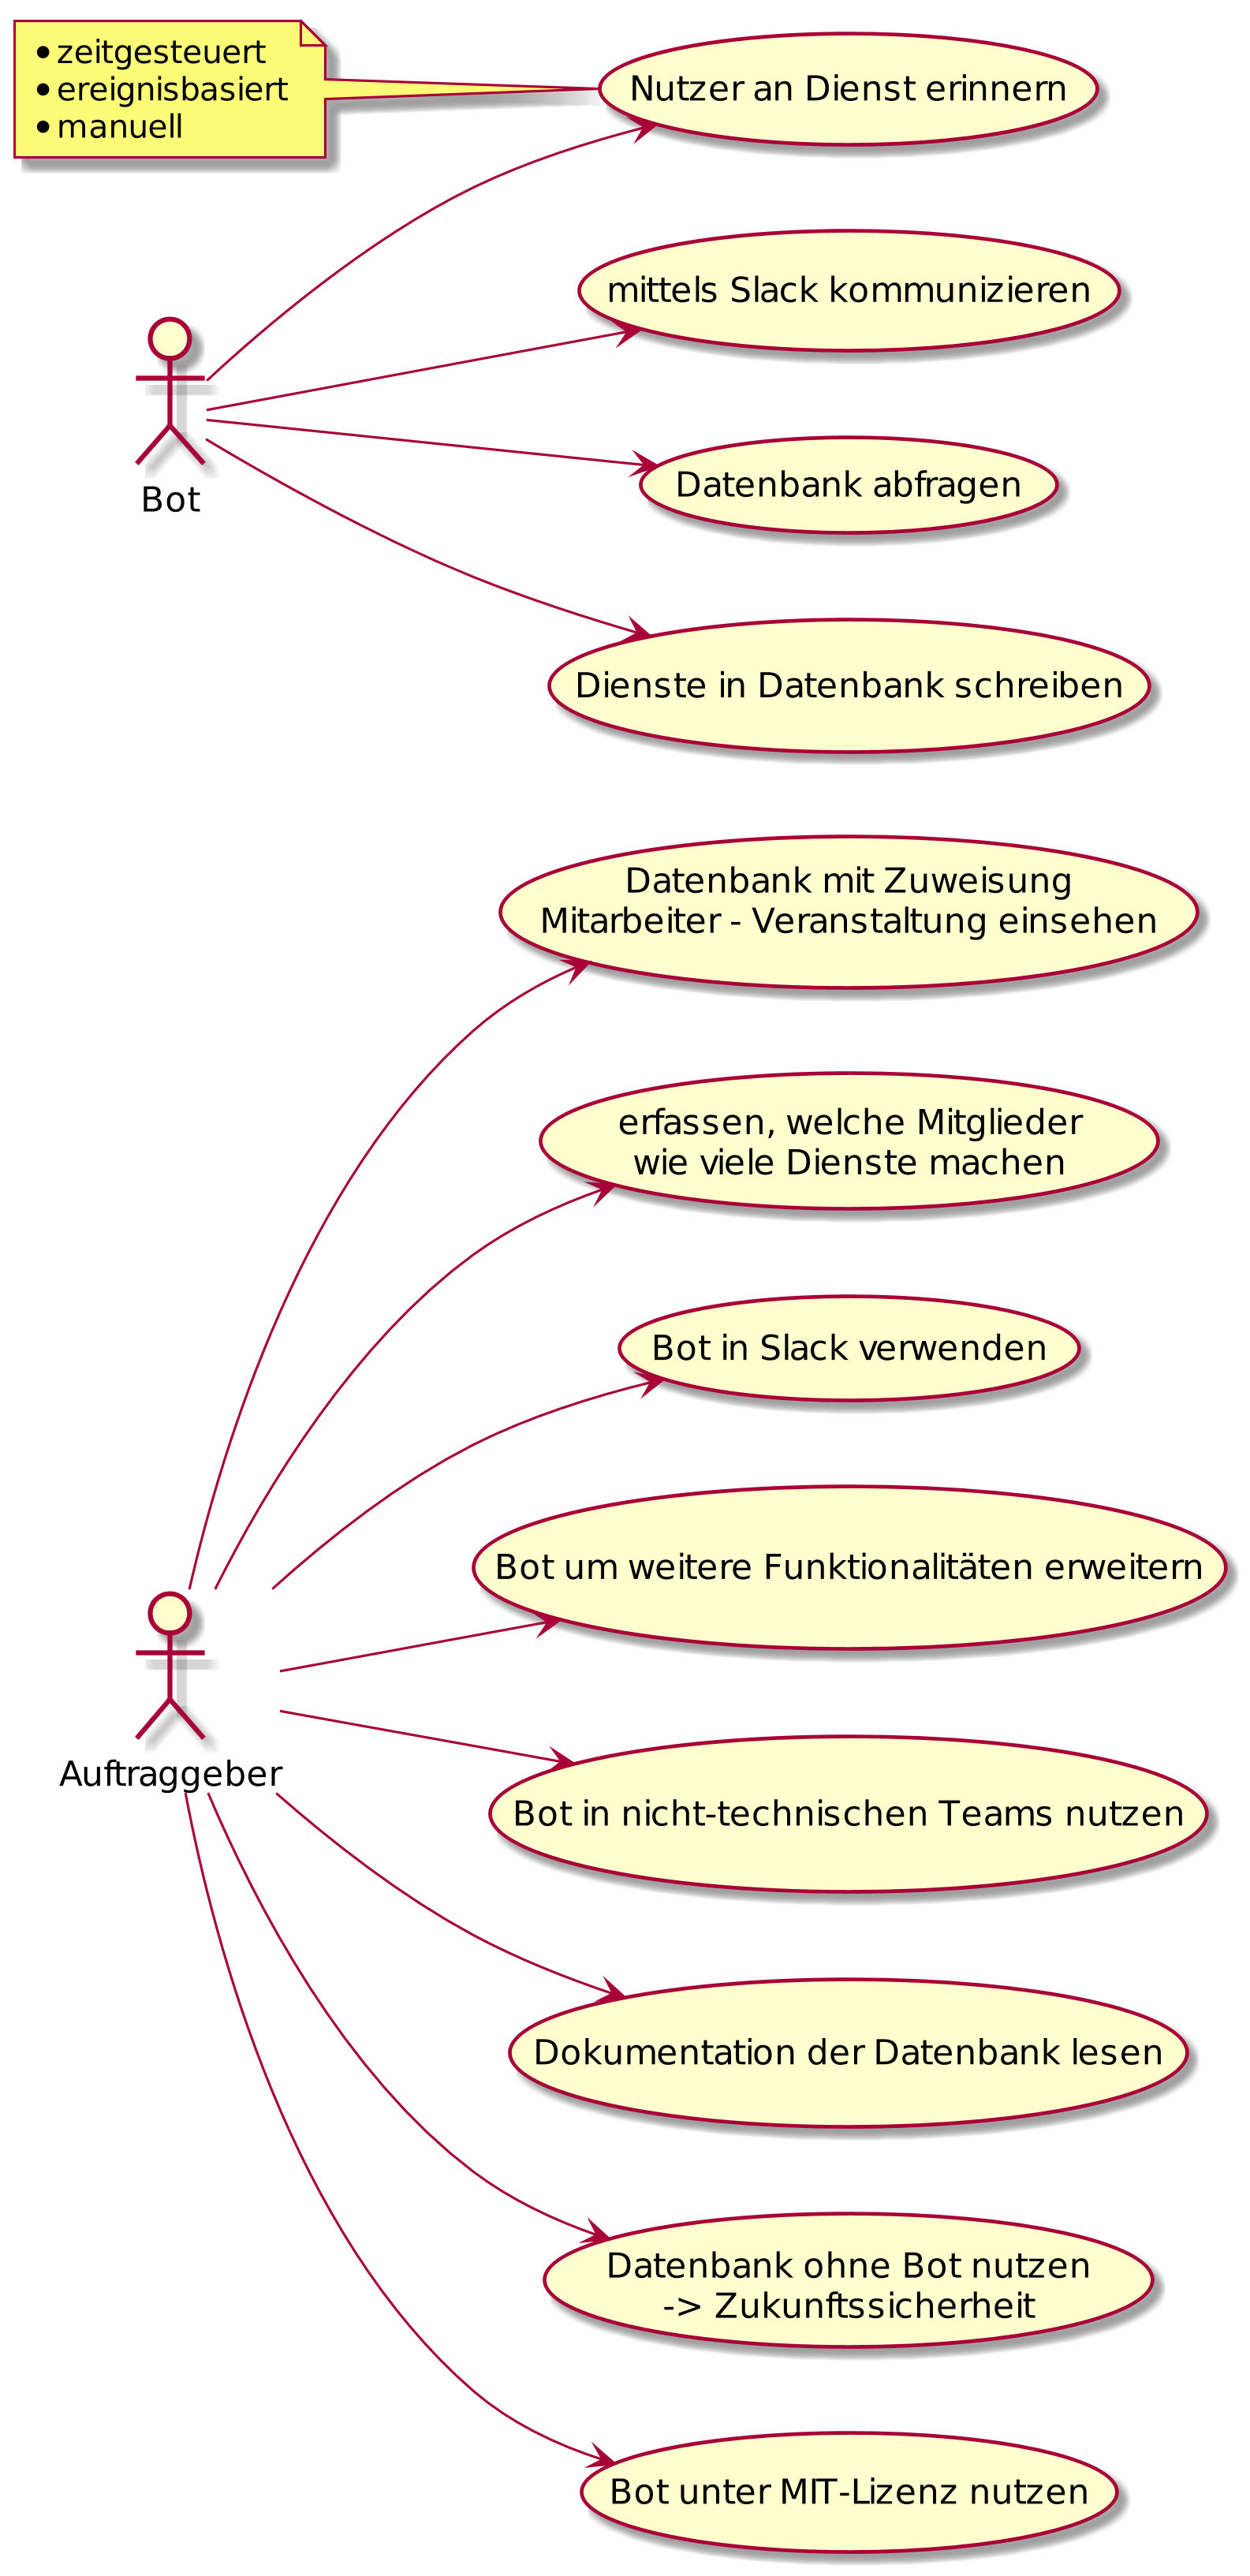
\includegraphics[width=0.7\textwidth]{../docs/uml/usecase-stakeholder.png}
    \caption{Anwendungsfalldiagramm für Auftraggeber und Bot}
    \label{usecase-auftrag}
\end{figure}


Für den zukünftigen Einsatz wurde ein weiteres Anwendungsfalldiagramm zur Unterteilung der Berechtigung der Nutzer erstellt. Gemäß Aufgabenstellung sind in \autoref{img:usecase-berechtigung} die Anwendungsfälle der Nutzer beschrieben. Die darin ebenfalls enthaltene Unterteilung der Berechtigungen dient hier nur der Vollständigkeit, da diese nicht zur initialen Aufgabenstellung gehört.
Eine weitere mögliche Betrachtung ist der unterschiedliche Grad an Fähigkeiten zwischen Administrator und Mitarbeiter. Während es einem Administrator zumutbar ist, beispielweise einen Nutzer direkt per Datenbankzugriff anzulegen, so benötigt der Mitarbeiter eine seinen Fähigkeiten angemessene Schnittstelle wie sie der Chatbot bieten soll.

\begin{figure}[htbp]
    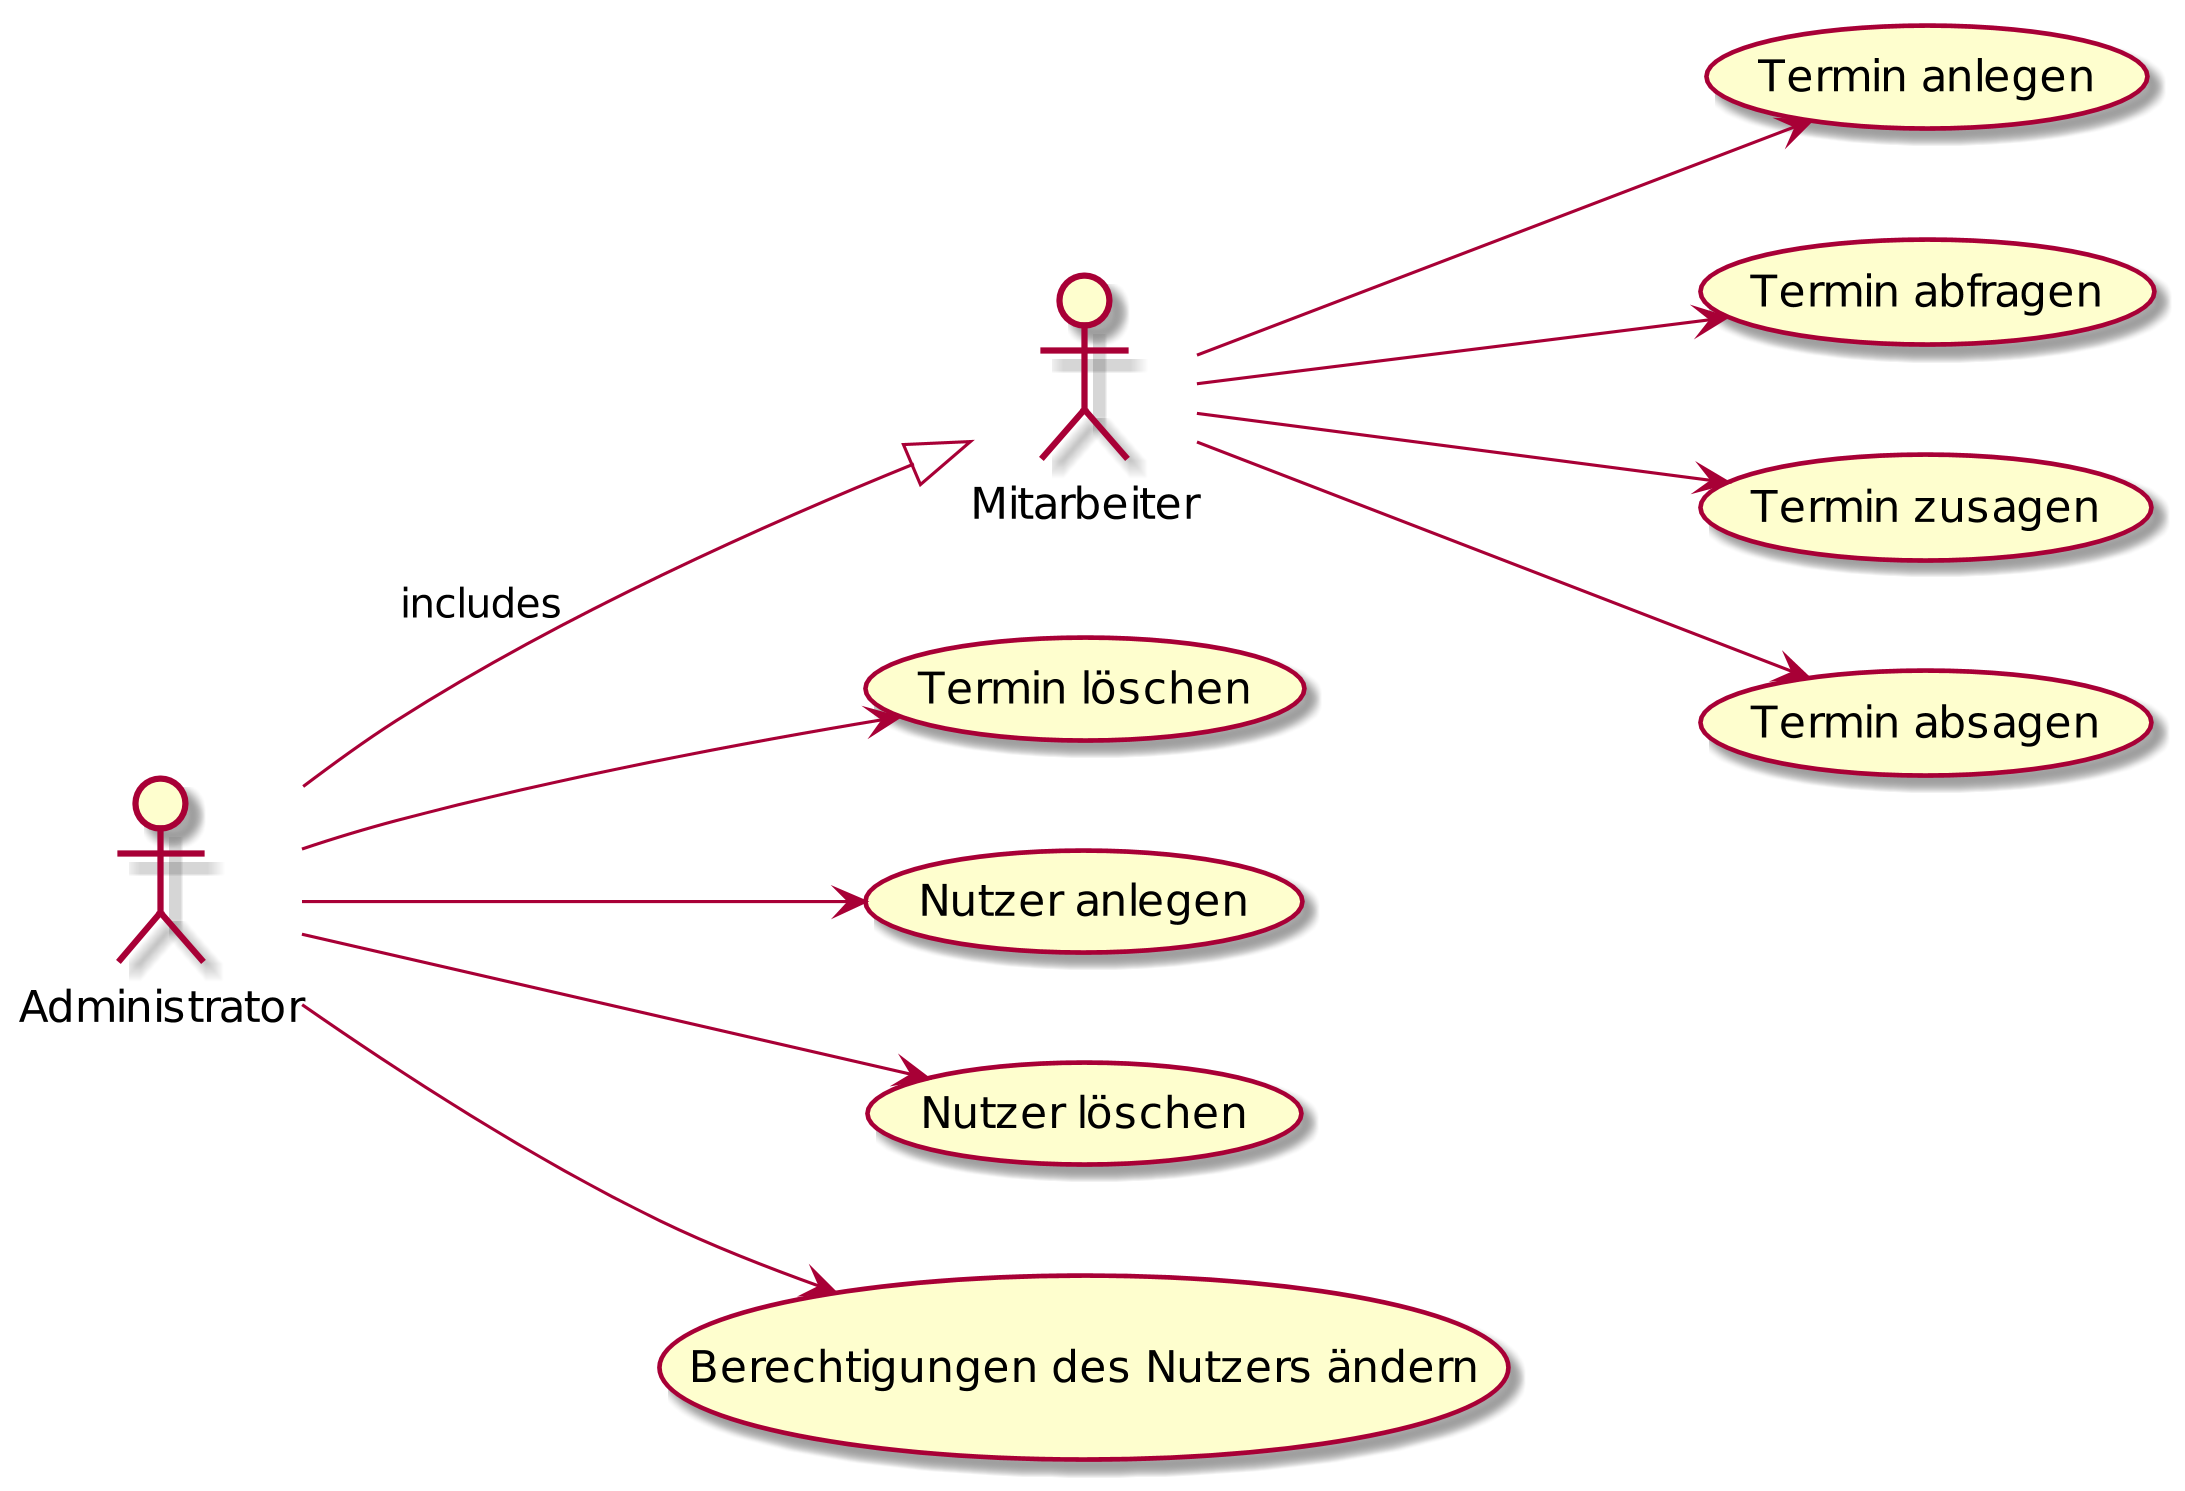
\includegraphics[width=0.9\textwidth]{../docs/uml/usecase-berechtigung.png}
    \caption{Anwendungsfalldiagramm zur Abgrenzung von Mitarbeiter und Administrator}
    \label{img:usecase-berechtigung}
\end{figure}